\chapter{Билет №11}

\section*{Аппаратные прерывания в Linux: запрос прерывания и линии IRQ. Простейшая схема аппаратной поддержки прерываний (концептуальная трех шинная архитектура системы). Быстрые и медленные прерывания, пример быстрого прерывания, флаги. Нижняя и верхняя половины обработчиков прерываний: регистрация обработчика аппаратного прерывания, функция регистрации и ее параметры. Нижние половины: softirq, tasklet, work queue — особенности реализации и выполнения в SMP-системах. Примеры, связанные с планированием отложенных действий (лаб. раб.)}

\textbf{ОС - аппаратно-зависимое ПО.}

\section{Система прерываний}

Система прерываний включает в себя:
\begin{enumerate}
  \item Системные вызовы (синхронные --- возникают в процессе выполнения программы, вызываются соответствующей командой).
  \item Исключения (синхронные --- возникают в процессе выполнения программы, переполнение стека/деление на 0...).
  \item Аппаратные прерывания (асинхронные --- не зависят ни от каких действий в системе, выполняются на высоких уровнях приоритетов, их выполнение нельзя прервать, задача --- информирование процессов о событиях в системе, от системного таймера/клавиатуры..., виды: от системного таймера (единственное периодическое), от действий оператора (ктрл+с), от внешних устройств).
\end{enumerate}

\textbf{Про таблицы прерываний:}

\begin{quote}  
  В 16-разрядной ОС (DOS) существует таблица векторов прерываний --- таблица, содержащая векторы прерывания (far-адреса обработчиков прерывания --- сегмент (2б) + смещение (2б)). Она начинается с нулевого адреса, занимает 1 Мб. Вектор прерывания - смещение в этой таблице.
  
  В 32-разрядной ОС cуществует IDT (Interrupt Descriptor Table), нужная для получения адресов обработчиков прерываний, содержащая 8-байтовые дескрипторы прерываний, хранящие информацию о смещении к обработчику прерывания в соответствующем сегменте.
  
  В 64-разрядной ОС существует IDT и список прерываний --- запутанная система.
  
  В современных системах часть перываний относится к APIC, а часть к подсистеме ОС MSI (Message Signal Interrupts).
\end{quote}

\section{Прерывания в последовательности ввода-вывода --- обслуживание запроса процесса на ввод-вывод}

\begin{table}[h!]
  \centering
  \begin{tabular}{p{1\linewidth}}
    \centering
    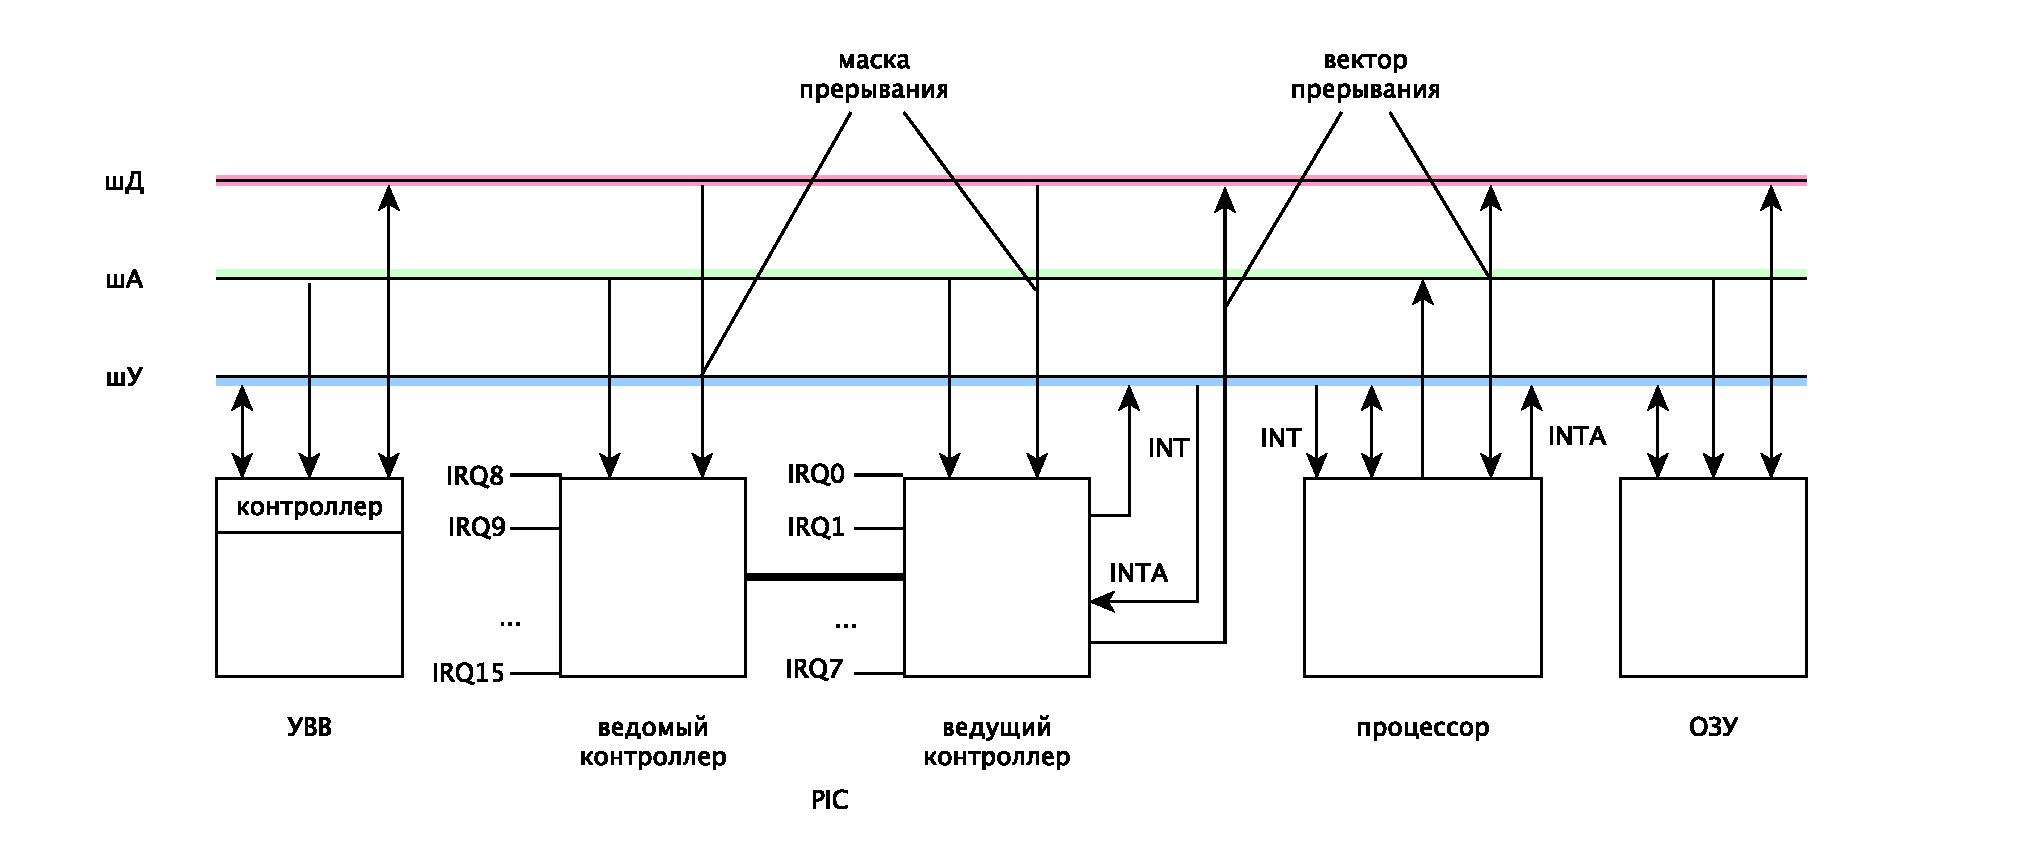
\includegraphics[width=0.9\linewidth]{./images/buses.pdf}
  \end{tabular}
\end{table}

Взаимодействие компьютера с внешними устройствами выполняется с помощью аппаратных прерываний --- идея распараллеливания действий, когда управление внешним устройством берёт на себя контроллер устройства (замена опроса готовности ВУ).

Взаимодействие компьютера с внешними устройствами выполняется с помощью аппаратных прерываний --- идея распараллеливания действий, когда управление внешним устройством берёт на себя контроллер устройства (замена опроса готовности ВУ).

\begin{enumerate}
  \item Запрос приложения на ввод/вывод переводит систему в режим ядра.
  \item Подсистема ввода/вывода вызывает драйвер устройства (в драйвере есть 1 обработчик прерывания от данного устройства).
  \item По окончании операции ввода/вывода контроллер устройства формирует сигнал прерывания, приходящий на соответствующую линию прерывания контроллера прерываний.
  \item Контроллер формирует сигнал INT, который по ШУ идёт на выделенную ножку процессора.
  \item В конце цикла выполнения каждой команды (выборка-дешифрирование-выполнение) процессор проверяет наличие сигнала на ножке. Если есть сигнал, процессор выставляет на ШУ INTA.
  \item Контроллер отправляет по ШД вектор прерывания в регистры процессора.
  \item Процессор смещается относительно нулевого адреса и находит в таблице адрес обработчика.
  \item Процессор по шине данных отправляет в контроллер маску прерываний, \sout{и контроллер адресуется по шине адреса}. 
\end{enumerate}

\begin{table}[h!]
  \centering
  \begin{tabular}{p{1\linewidth}}
    \centering
    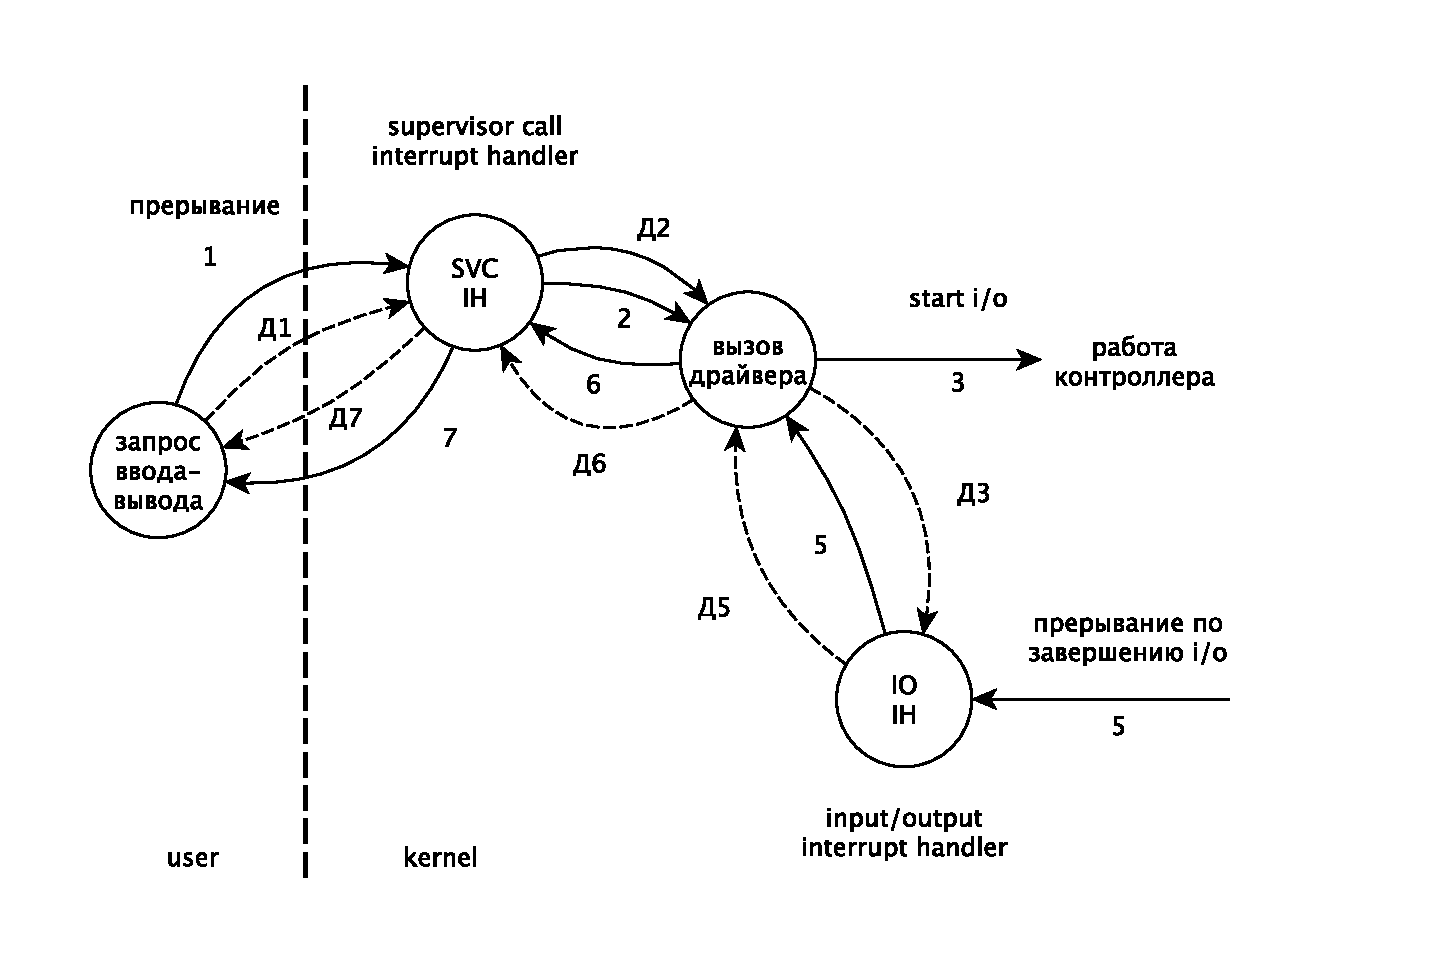
\includegraphics[width=0.8\linewidth]{./images/driver.pdf}
  \end{tabular}
\end{table}

\section{Обработчики аппаратных прерываний: регистрация в системе --- функция и ее параметры, примеры}

Основная задача обработчика прерывания --- передача данных от устройства по шине данных, если была запрошена операция чтения. Даже если была запрошена операция записи, устройство все равно оправляет по шине данных информацию об успешности операции. Чтобы обработать ее, обработчик должен сохранять информацию, поступающую от устройства в буфер ядра. Затем эта информация поступит приложению, запросившему ввод/вывод.

\section{Обработка аппаратных прерываний}
Любые аппаратные прерывания выполняются на самом высоком уровне приоритета (самый высокий --- системный таймер, выше него только migration для перебалансировки нагрузки между процессорами и power при падении напряжения --- система отключается от питания и не может работать).

Далее идут остальные прерывания от внешних устройств.

Т.к. АП -- важнейшие прерывания в системе, то для того, чтобы исключить негативные ситуации, связанные с обработкой данных, поступивших от внешних устройств(в многопроцессорных системах), система делает следующее:

Т.к. любое АП не может обрабатываться всеми ядрами(обрабатывается определенным ядром), то на этом ядре все прерывания запрещаются, а в системе запрещаются все прерывания по конкретной линии IRQ.

\section{Нижняя и верхняя половины обработчиков прерываний}

АП не могут выполнять большой объем действий, т.е. выполняться длительное время, т.к. никакая другая работа на данном процессоре выполняться не может, что негативно сказывается на \textbf{производительности и отзывчивости системы}.

Эти 2 части --- top\_half и bottom\_half. top\_half (interrupt handler) копирует данные устройства в специальный буфер, инициализирует отложенное действие bottom\_half (softirq, tasklet или workqueue) и завершается. top\_half должен выполниться быстро, так как при этом игнорируются остальные прерывания. bottom\_half выполняется при разрешённых остальных прерываниях и делает всю остальную обработку прерывания.

\section{Быстрые и медленные прерывания}

Выделяются быстрые и медленные аппаратные прерывания. Быстрые --- выполняются атомарно, не делятся на части, в современных системах это только прерывание от системного таймера. Медленные --- все остальные, делятся на 2 части.

Если речь идет о медленных, то одной из задач обработчика АП является инициализация отложенного действия в виде softirq, tasklet, workqueue.

bottom\_half --- отложенные действия, при этом этими отложенными действиями система управляет по-разному.

\section{Функция регистрации и ее параметры}

Система предоставляет разработчику возможность зарегистрировать собственный обработчик прерывания.

Для этого ядро предоставляет функцию request\_irq

\begin{lstlisting}
  typedef irqreturn_t (*irq_handler_t)(int, void *); 
  
  int request_irq(unsigned int irq, irq_handler_t handler, unsigned long flags, const char* name, void *dev);
\end{lstlisting}

irq --- номер линии прерывания. handler --- обработчик прерывания. flags --- флаги. name --- имя обработчика. dev - указатель на некоторый объект, используется для освобождения линии прерывания от указанного обработчика:

\begin{lstlisting}
  const void *free_irq(unsigned int irq, void *dev_id);
\end{lstlisting}

\section{Флаги}
\begin{enumerate}
        \item level\_triggered, edge\_triggered --- определяют срабатывание;           
  \item IRQF\_SHARED --- разрешает разделение линии irq между несколькими обработчиками прерываний.
  \item IRQF\_PROBE\_SHARED --- устанавливается абонентом, если предполагается возможность проблем/нестыковок при разделении.
  \item IRQF\_TIMER --- определяет единственное быстрое прерывание.
  \item IRQF\_PERCPU --- закрепление конкретного прерывания за определенным процессом (монопольно).
\end{enumerate}

\section{Тасклеты --- объявление, планирование}

Тасклет --- специальный тип softirq. Тасклеты представлены двумя типами отложенных прерываний: HI\_SOFTIRQ (вып. раньше)  и TASKLET\_SOFTIRQ.

\textbf{Тасклет не может выполняться параллельно, выполняется атомарно на том же процессоре, на котором выполняется обработчик запланировавшего его прерывания. Инициализируется как статически, так и динамически. Выполняется в контексте прерывания --- нельзя использовать средства взаимоисключения, кроме spinlocks (активное ожидание на процессоре). Выполняется ksofirqd. Является упрощённым интерфейсом softirq.}

Определена структура:

\begin{lstlisting}
struct tasklet_struct
{
	struct tasklet_struct *next; // указатель на следующий тасклет в односвязном  списке
	unsigned long state; // состояние тасклета
	atomic_t count; // счетчик ссылок 
	bool use_callback; // флаг
	union {
		void (*func)(unsigned long data); // функция-обработчик тасклета
		void (*callback)(struct tasklet_struct *t);
	};
	unsigned long data; // аргумент функции-обработчика тасклет
};
\end{lstlisting}

Тасклеты в отличие от softirq могут быть зарегистрированы как статически, так и динамически. Статически тасклеты создаются с помощью двух макросов (man 6.2.1):

\begin{lstlisting}
#define DECLARE_TASKLET(name, _callback)		\
struct tasklet_struct name = {				\
	.count = ATOMIC_INIT(0),			\
	.callback = _callback,				\
	.use_callback = true,				\
}
#define DECLARE_TASKLET_DISABLED(name, _callback)	\
struct tasklet_struct name = {				\
	.count = ATOMIC_INIT(1),			\
	.callback = _callback,				\
	.use_callback = true,				\
}
\end{lstlisting}

Оба  макроса статически создают экземпляр структуры struct tasklet\_struct с указанным именем (name). Например,

\begin{lstlisting}
DECLARE_TASKLET(my_tasklet, tasklet_handler);
\end{lstlisting}

Эта строка эквивалентна следующему объявлению:
\begin{lstlisting}
struct tasklet_struct my_tasklet = {NULL, 0, ATOMIC_INIT(0), tasklet_handler};
\end{lstlisting}

В данном примере создается тасклет с именем my\_tasklet, который разрешен для выполнения. Функция tasklet\_handler будет обработчиком этого тасклета. Поле dev отсутствует в текущих ядрах.

При динамическом создании тасклета объявляется указатель на
struct tasklet\_struct, а затем для инициализации вызывается функция:
\begin{lstlisting}
extern void tasklet_init(struct tasklet_struct *t, void (*func)(unsigned long), unsigned long data);
\end{lstlisting}

Пример:
\begin{lstlisting}
tasklet_init(t, tasklet_handler, data);
\end{lstlisting}   

Тасклеты должны быть зарегестрированы для выполнения. Тасклеты могут быть запланированы на выполнение функциями:
\begin{lstlisting}
tasklet_schedule(struct tasklet_struct *t); 
tasklet_hi_shedule(struct tasklet_struct *t);
\end{lstlisting}  

Когда тасклет запланирован, ему выставляется состояние TASKLET\_STATE\_SCHED, и он добавляется в очередь. Пока он находится в этом состоянии, запланировать его еще раз не получится, т.е. в этом случае просто ничего не произойдет. Тасклет не может находиться сразу в нескольких местах очереди на планирование, которая организуется через поле next структуры tasklet\_struct. После того, как тасклет был запланирован, он выполниться только один раз.

Свойства:
\begin{enumerate}
	\item Если вызывается функция tasklet\_schedule(), то после этого тасклет гарантированно будет выполнен на каком-либо процессоре хотя бы один раз. 
	\item Если тасклет уже запланирован, но его выполнение все еще не запущено, он будет выполнен только один раз. 
	\item Если этот тасклет уже запущен на другом процессоре (или schedule вызывается из самого тасклета), выполнение переносится на более поздний срок. 
	\item Если разработчик считает, что в данном тасклете нужно выполнить действия, которые могут выполняться в других таскоетах, он реализует взаимоисключение с помощью spinlocks.
\end{enumerate}

\begin{table}[H]
\begin{center}
\begin{tabular}{|c|l|l|l|}
\hline
Критерии                                                            & \multicolumn{1}{c|}{softirq}                                                               & \multicolumn{1}{c|}{tasklet}                                                                    & \multicolumn{1}{c|}{workqueue}                                                           \\ \hline
Определение                                                         & \begin{tabular}[c]{@{}l@{}}10 шт. определено\\ в ядре статически\end{tabular}              & С + Д                                                                                           & С + Д                                                                                    \\ \hline
Взаимоискл.                                                        & Да                                                                                         & Нет                                                                                             & Да                                                                                       \\ \hline
\begin{tabular}[c]{@{}c@{}}Возможность \\ паралл. вып.\end{tabular} & Да                                                                                         & Нет                                                                                             & Да                                                                                       \\ \hline
Выполнение                                                          & \begin{tabular}[c]{@{}l@{}}В контексте спец.\\ потоков ядра (ksoftirqd)\end{tabular} & \begin{tabular}[c]{@{}l@{}}В контексте\\ запланировавшего\\ обраб. прерыв.\end{tabular} & \begin{tabular}[c]{@{}l@{}}В контексте спец.\\ потоков ядра (kworker)\end{tabular} \\ \hline
Блокируются                                                         & Наверное нет                                                                                        & Нет                                                                                             & Да                                                                                       \\ \hline
\end{tabular}
\end{center}
\end{table}

\section{spin\_lock}

Race condition --- условия гонок: процессы выполняются с разной скоростью и пытаются получить доступ к разделяемым переменным. 

Аппаратная реализация взаимоисключения --- test\_and\_set. Атомарная функция, реализующая как неделимое действие проверку и установку значения в памяти. По сути, читает значение переменной b, копирует его в a, устанавливает b значение true. Считается, что это не приведет к бесконечному откладыванию. 

Использование test\_and\_set в цикле проверки значения переменной называется циклической блокировкой. Spin-блокировки --- активное ожидание на процессоре (время непроизводительно расходуется на проверку флага другого процессора). Реализация test\_and\_set связана с блокировкой локальной шины памяти, в результате один поток может занять шину на длительное время, что понижает отзывчивость (решение --- 2 вложенных цикла, если переменная занята --- выполняется обычный цикл без блокировки шины).

\begin{lstlisting}
	void spin_lock(spin_lock_t* c)
	{
		while (test_and_set(*c) != 0)
		{
			/* ресурс занят */
			
			/*
			while (*c != 0) 
			{
			...
			}
			*/
		}
	}
	
	void spin_unlock(spin_lock_t* c)
	{
		*c = 0;
	}
\end{lstlisting}

Циклическую блокировку может удерживать только 1 поток. Захваченная --- в состоянии contended. Если другой поток пытается захватить уже захваченную, то блокировка находится в состоянии конфликта, а поток выполняет цикл проверки busy\_loop. Блокировка должна быть связана с тем, что она блокирует. Запрещаются данные (разделяемый ресурс), а не код. В этой блокировке есть смысл, только когда ее длительность не превышает 2 переключений контекста.

\textbf{Пример из лабораторной:}

\begin{lstlisting}
#include <linux/kernel.h>
#include <linux/module.h>
#include <linux/interrupt.h>
#include <linux/slab.h>
#include <asm/io.h>

#include "ascii.h"

#define IRQ_NUMBER 1

MODULE_LICENSE("GPL");
MODULE_AUTHOR("Karpova Ekaterina");

struct tasklet_struct *tasklet;
char tasklet_data[] = "key pressed";

void tasklet_func(unsigned long data)
{
    printk(KERN_INFO "+: -----------------------");
    printk(KERN_INFO "+: tasklet began");
    printk(KERN_INFO "+: tasklet count = %u", tasklet->count.counter);
    printk(KERN_INFO "+: tasklet state = %lu", tasklet->state);

    printk(KERN_INFO "+: key code - %d", data);
    if (data < ASCII_LEN)
        printk(KERN_INFO "+: key press - %s", ascii[data]);
    if (data > 128 && data < 128 + ASCII_LEN)
        printk(KERN_INFO "+: key release - %s", ascii[data - 128]);
        
    printk(KERN_INFO "+: tasklet ended");
    printk(KERN_INFO "+: -----------------------");
}

static irqreturn_t my_irq_handler(int irq, void *dev_id)
{
  int code;
  printk(KERN_INFO "+: my_irq_handler called\n");
  
  if (irq != IRQ_NUMBER)
  {
    printk(KERN_INFO "+: irq not handled");
    return IRQ_NONE;
  }
  
  printk(KERN_INFO "+: tasklet state (before schedule) = %lu",
                 tasklet->state);
  code = inb(0x60);
  tasklet->data = code;
  tasklet_schedule(tasklet);
  printk(KERN_INFO "+: tasklet scheduled");
  printk(KERN_INFO "+: tasklet state (after schedule) = %lu",
                  tasklet->state);
                  
  return IRQ_HANDLED;
}

static int __init my_init(void) 
{
  if (request_irq(IRQ_NUMBER, my_irq_handler, IRQF_SHARED, "tasklet_irq_handler", (void *) my_irq_handler))
  {
    printk(KERN_ERR "+: cannot register irq handler\n");
    return -1;
  }
  
  tasklet = kmalloc(sizeof(struct tasklet_struct), GFP_KERNEL);

  if (tasklet == NULL)
  {
        printk(KERN_ERR "+: kmalloc error");
        return -1;
  }

  tasklet_init(tasklet, tasklet_func, (unsigned long)tasklet_data);
  
  printk(KERN_INFO "+: module loaded\n");
  return 0;
}

static void __exit my_exit(void)
{
  tasklet_kill(tasklet);
  free_irq(IRQ_NUMBER, my_irq_handler);

  printk(KERN_INFO "+: module unloaded\n");
}

module_init(my_init);
module_exit(my_exit);

\end{lstlisting}

\section{Очереди работ --- объявление, создание, постановка работы в очередь, планирование}

Очереди работ --- еще один тип bottom\_half (отложенного действия). Кроме очередей, которые мы создаём, есть общесистемные очереди и соответствующие возможности для работы с этими очередями. Определена структура в <linux/workqueue.h>.

\begin{lstlisting}
	struct workqueue_struct {
	struct list_head	pwqs;		/* WR: all pwqs of this wq */
	struct list_head	list;		/* PR: list of all workqueues */

	struct mutex		mutex;		/* protects this wq */
	int			work_color;	/* WQ: current work color */
	int			flush_color;	/* WQ: current flush color */
	atomic_t		nr_pwqs_to_flush; /* flush in progress */
	struct wq_flusher	*first_flusher;	/* WQ: first flusher */
	struct list_head	flusher_queue;	/* WQ: flush waiters */
	struct list_head	flusher_overflow; /* WQ: flush overflow list */

	struct list_head	maydays;	/* MD: pwqs requesting rescue */
	struct worker		*rescuer;	/* MD: rescue worker */

	int			nr_drainers;	/* WQ: drain in progress */
	int			saved_max_active; /* WQ: saved pwq max_active */

	struct workqueue_attrs	*unbound_attrs;	/* PW: only for unbound wqs */
	struct pool_workqueue	*dfl_pwq;	/* PW: only for unbound wqs */

#ifdef CONFIG_SYSFS
	struct wq_device	*wq_dev;	/* I: for sysfs interface */
#endif
#ifdef CONFIG_LOCKDEP
	char			*lock_name;
	struct lock_class_key	key;
	struct lockdep_map	lockdep_map;
#endif
	char			name[WQ_NAME_LEN]; /* I: workqueue name */

	/*
	 * Destruction of workqueue_struct is RCU protected to allow walking
	 * the workqueues list without grabbing wq_pool_mutex.
	 * This is used to dump all workqueues from sysrq.
	 */
	struct rcu_head		rcu;

	/* hot fields used during command issue, aligned to cacheline */
	unsigned int		flags ____cacheline_aligned; /* WQ: WQ_* flags */
	struct pool_workqueue __percpu *cpu_pwqs; /* I: per-cpu pwqs */
	struct pool_workqueue __rcu *numa_pwq_tbl[]; /* PWR: unbound pwqs indexed by node */
};
\end{lstlisting}

На процессор имеется 2 kworker: normal и high. Это соответствует созданию очередей с нормальным и высоким уровнем приоритета, вторые будут выполняться раньше, но это разные воркеры.

worker --- рабочий поток ядра (worker\_thread).

Все воркеры выполняются как обычные потоки ядра, при этом они выполняют функцию worker\_thread().
\begin{enumerate}
	\item После инициализации worker\_thread() она входит в бесконечный цикл и засыпает (прерываемый сон).
	\item Она просыпается, когда в очередь ставится какая-то работа и начинает выполнять ее.
	\item Закончив выполнение работы, поток опять засыпает.
\end{enumerate}

В системе также есть структура

\begin{lstlisting}
/*
* Очередь отложенных действий, связанная с процессором:
*/
struct cpu_workqueue_struct 
{
   spinlock_t lock; /* Очередь для защиты данной структуры */
   long remove_sequence; /* последний добавленный элемент
  (следующий для запуска ) */
   long insert_sequence; /* следующий элемент для добавления */
   struct list_head worklist; /* список действий на каждое cpu */
   wait_queue_head_t more_work;
   wait_queue_head_t work_done;
  struct workqueue_struct *wq; /* соответствующая структура
                                workqueue_struct */
    task_t *thread; /* соответствующий поток (функция) */
    int run_depth; /* глубина рекурсии функции run_workqueue() */
};
\end{lstlisting}

Иллюстрация для cpu0 (для всех cpu одинаково):

\begin{table}[h!]
  \centering
  \begin{tabular}{p{1\linewidth}}
    \centering
    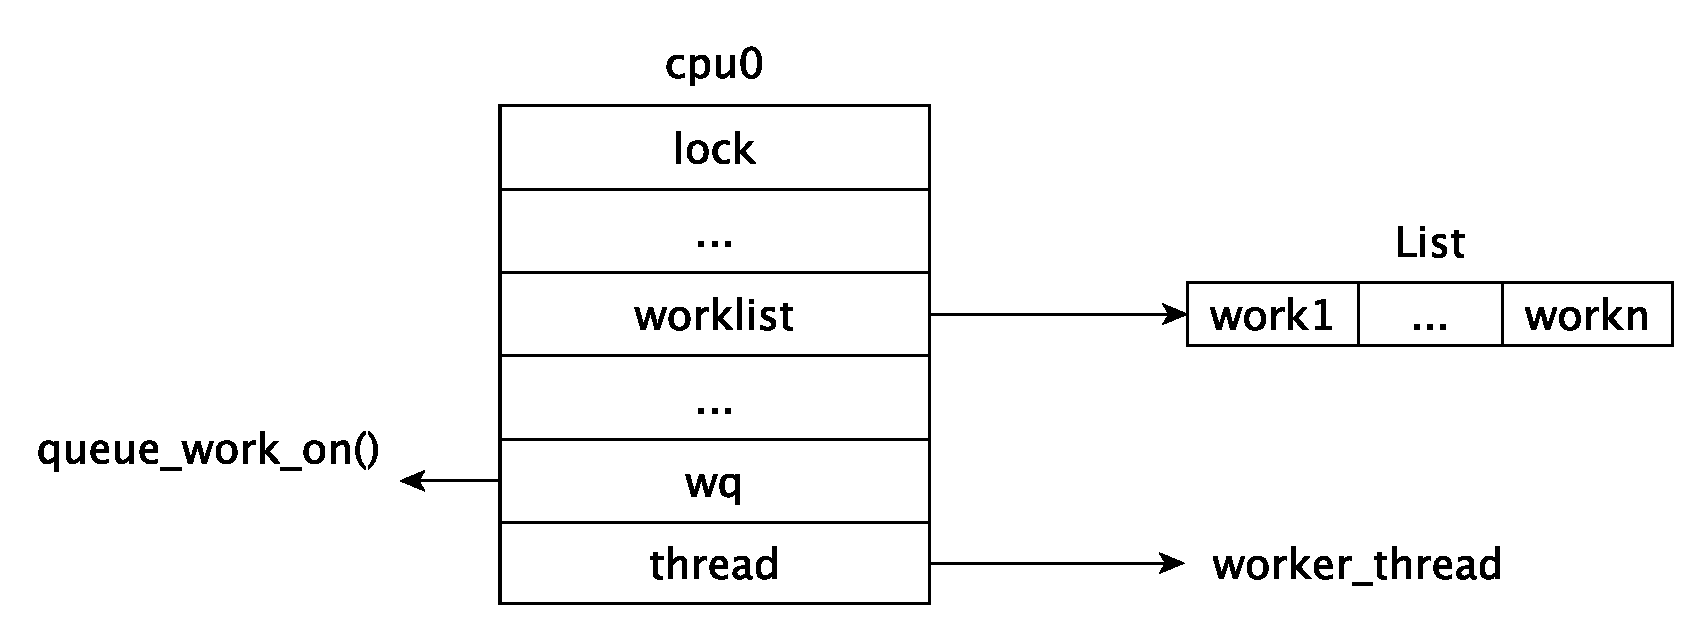
\includegraphics[width=0.8\linewidth]{./images/cpu0.pdf}
  \end{tabular}
\end{table}

wq --- указатель на инициализированную структуру очереди работ.

Работа описывается структурой (1 экземпляр на каждое отложенное действие):

\begin{lstlisting}
typedef void (*work_func_t) (struct work_struct *work);
	struct work_struct {
        atomic_long_t data;
        struct list_head entry;
        work_func_t func; // обработчик работы
#ifdef CONFIG_LOCKDEP
        struct lockdep_map lockdep_map;
#endif
};
\end{lstlisting}

В современных системах очередь работ создается функцией alloc\_workqueue():

\begin{lstlisting}
	struct workqueue_struct *alloc_workqueue(const char *fmt,
					 unsigned int flags,
					 int max_active, ...);
\end{lstlisting}

fmt - формат на имя очереди (workqueue), но в отличие от старых реализаций потоков с этим именем не создается. flags - флаги определяют как очередь работ будет выполняться. max\_active - ограничивает число задач (work) из некоторой очереди, которые могут выполняться одновременно на любом CPU.

Кроме этой, есть еще функция:
\begin{lstlisting}
	#define alloc_ordered_workqueue(fmt, flags, args...)			\
	alloc_workqueue(fmt, WQ_UNBOUND | __WQ_ORDERED |		\
			__WQ_ORDERED_EXPLICIT | (flags), 1, ##args)
\end{lstlisting}

create\_workqueue() --- устаревшая.

Несколько объектов, связанных с очередью работ (workqueue), представлены в ядре соответствующими структурами:
\begin{enumerate}
	\item Работа (work);
	\item Очередь работ (workqueue) – коллекция work. Workqueue и work относятся как один-ко-многим;
	\item Рабочий (worker). Worker соответствует потоку ядра worker\_thread;
	\item Пул рабочих потоков (worker\_pool) это – набор рабочих (worker). Worker\_pool и worker относятся как «один ко многим»;
	\item Pwd (pool\_workqueue) это – посредник, который отвечает за отношение workqueue и worker\_pool: workqueue и pwd является отношением один-ко-многим, а pwd и worker\_pool – отношение один-к-одному.
\end{enumerate}

\begin{quote}
	Для начала пулы для привязанных очередей (на картинке). Для каждого CPU статически выделяются два worker pool: один для высокоприоритетных work’ов, другой — для work’ов с нормальным приоритетом. То есть, если ядра у нас четыре, то привязанных пулов будет всего восемь, не смотря на то, что workqueue может быть сколько угодно.

Когда мы создаем workqueue, у него для каждого CPU выделяется служебный pool\_workqueue (pwq). Каждый такой pool\_workqueue ассоциирован с worker pool, который выделен на том же CPU и соответствует по приоритету типу очереди. Через них workqueue взаимодействует с worker pool.

Worker’ы исполняют work’и из worker pool без разбора, не различая, к какому workqueue они принадлежали изначально.

Для непривязанных очередей worker pool’ы выделяются динамически.
\end{quote}

\section{Флаги}

\begin{enumerate}
	\item WQ\_UNBOUND --- очередь работ не связана ни с каким cpu.
	\item WQ\_FREEZABLE --- очередь работ может блокироваться.
	\item WQ\_HIGHPRI --- задания, представленные в такую очередь, будут поставлены в начало очереди и будут выполняться (почти) немедленно.
	\item WQ\_CPU\_INTENSIVE --- очередь работ может интенсивно использовать процессор.
	\item WQ\_POWER\_EFFICIENT --- очереди работ, связанные с конкретным процессором, являются более предпочтительными, так как имеют более высокую производительность благодаря локальному кешу. Но такая привязанность к конкретному процессору имеет отрицательный побочный эффект --- увеличение энергопотребления.
\end{enumerate}

Продолжение про WQ\_POWER\_EFFICIENT

Это связано с тем, что если энергия не тратится, процессор простаивает.

Такие соображения учитываются в любой системе.

Таким образом, если нет workqueue, привязанных к конкретному процессору, можно «не трогать» этот неработающий процессор и, если позволяют соответствующие условия, выполнять эту работу на том процессоре, который работает.

Фактически мы можем ограничиться одним процессором...

\section{Создание работы}
\par Мы создаем очередь работ для того, чтобы поместить в нее нужные нам действия (работы). 

\par Существует статический способ определения работы с помощью макроса

\begin{lstlisting}[language=C, label=lst:1, caption=Статический способ определения]
DECLARE_WORK(name, void (*func)(void*));
struct work_struct *name; // имя (экземпляра) структуры work_struct
\end{lstlisting}

func -- имя функции, которая вызывается из workqueue (код для выполнения отложенных действий, нижняя половина).

\par Работу можно определить динамически т.е. в процессе выполнения программы:

\begin{lstlisting}[language=C, label=lst:1, caption=Динамический способ определения]
#define INIT_WORK(_work, func) __INIT_WORK((_work,(func), 0)
\end{lstlisting}

\begin{quote}
\begin{lstlisting}[language=C, label=lst:1, caption=Определение \_\_INIT\_WORK()]
__INIT_WORK((_work, _func, _onstack)
do {
    ...
    INIT_LIST_HEAD(&(work)->entry);
    (_work)->func=(-func);
} while (0);
\end{lstlisting}
\end{quote}

\begin{quote}
Также может встретиться функция PREPARE\_WORK(). INIT\_WORK() производит инициализацию работ более тщательно (советую Вам использовать её), а PREPARE\_WORK() используется, если работа была инициализирована, для сокращения времени повторной инициализации.
\end{quote}

\section{Постановка работы в очередь}

Работа поставлена в очередь —- она попадает в список и через какое-то время (не мгновенно) будет выполнена.

Инициализировав работу, требуется поставить ее в очередь. Это делает функция:
\begin{lstlisting}
bool queue_work(struct workqueue_struct *queue, struct work_struct *work);
\end{lstlisting}

queue — очередь, в которую мы хотим поставить работу;
work — инициализированная структура work\_struct.

Также есть
\begin{lstlisting}
bool queue_delayed_work(..., unsigned long delay); // ... - те же два параметра
\end{lstlisting}

delay — время, через которое данная работа может быть поставлена в очередь.
Определяет количество jiffes («мгновений»).

queue\_work() определена через queue\_work\_on().

\section{Завершение работы/очереди работ}

Принудительное завершение очереди работ:
\begin{lstlisting}
extern void _flush_workqueue(struct worqueue_struct *wq);
\end{lstlisting}

Принудительно завершить работу и блокировать прочую обработку прежде, чем работа будет закончена:
\begin{lstlisting}
extern bool flush_work(struct work_struct *work);
\end{lstlisting}

Чтобы абсолютно точно отменить выполнение (отменить работу, если она еще не выполнена обработчиком; завершит работу в очереди, либо возникнет блокировка до тех пор, пока не будет завершен обратный вызов (если работа уже выполняется обработчиком)), советуют использовать:
\begin{lstlisting}
extern bool cancel_work(...);
\end{lstlisting}

Если работа отложена, вы можете использовать функции flush\_delayed\_work() и \\ cancel\_delayed\_work().

\textbf{Пример:}

\begin{lstlisting}
#include <linux/module.h>
#include <linux/kernel.h>
#include <linux/interrupt.h>
#include <linux/slab.h>
#include <asm/io.h>
#include <linux/stddef.h>
#include <linux/workqueue.h>
#include <linux/delay.h>

#include "ascii.h"

#define IRQ_NUMBER 1

MODULE_LICENSE("GPL");
MODULE_AUTHOR("Karpova Ekaterina");

typedef struct
{
    struct work_struct work;
    int code;
} my_work_struct_t;

static struct workqueue_struct *my_wq;

static my_work_struct_t *work1;
static struct work_struct *work2;

void work1_func(struct work_struct *work)
{
    my_work_struct_t *my_work = (my_work_struct_t *)work;
    int code = my_work->code;

    printk(KERN_INFO "+: -----------------------");
    printk(KERN_INFO "+: work1 began");

    printk(KERN_INFO "+: key code - %d", code);
    if (code < ASCII_LEN)
        printk(KERN_INFO "+: key press - %s", ascii[code]);
    if (code > 128 && code < 128 + ASCII_LEN)
        printk(KERN_INFO "+: key release - %s", ascii[code - 128]);

    printk(KERN_INFO "+: work1 ended");
    printk(KERN_INFO "+: -----------------------");
}

void work2_func(struct work_struct *work)
{
    printk(KERN_INFO "+: -----------------------");
    printk(KERN_INFO "+: work2 began");
    msleep(10);
    printk(KERN_INFO "+: work2 ended");
    printk(KERN_INFO "+: -----------------------");
}

irqreturn_t my_irq_handler(int irq, void *dev)
{
    int code;
    printk(KERN_INFO "+: my_irq_handler called\n");

    if (irq != IRQ_NUMBER)
    {
        printk(KERN_INFO "+: irq not handled");
        return IRQ_NONE;
    }

    code = inb(0x60);
    work1->code = code;

    queue_work(my_wq, (struct work_struct *)work1);
    queue_work(my_wq, work2);

    return IRQ_HANDLED;
}

static int __init my_init(void)
{
    int rc = request_irq(IRQ_NUMBER, my_irq_handler, IRQF_SHARED,
                      "work_irq_handler", (void *) my_irq_handler);
    if (rc) {
        printk(KERN_ERR "+: cannot register irq handler");
        return rc;
    }

    my_wq = alloc_workqueue("%s", __WQ_LEGACY | WQ_MEM_RECLAIM, 1, "my_wq");
    if (my_wq == NULL)
    {
        printk(KERN_ERR "+: cannot alloc workqueue");
        return -1;
    }

    work1 = kmalloc(sizeof(my_work_struct_t), GFP_KERNEL);
    if (work1 == NULL)
    {
        printk(KERN_ERR "+: cannot alloc work1");
        destroy_workqueue(my_wq);
        return -1;
    }

    work2 = kmalloc(sizeof(struct work_struct), GFP_KERNEL);
    if (work2 == NULL)
    {
        printk(KERN_ERR "+: cannot alloc work2");
        destroy_workqueue(my_wq);
        kfree(work1);
        return -1;
    }

    INIT_WORK((struct work_struct *)work1, work1_func);
    INIT_WORK(work2, work2_func);
    
    printk(KERN_INFO "+: module loaded");

    return 0;
}

static void __exit my_exit(void)
{
    synchronize_irq(IRQ_NUMBER);
    free_irq(IRQ_NUMBER, my_irq_handler);

    flush_workqueue(my_wq);
    destroy_workqueue(my_wq);
    kfree(work1);
    kfree(work2);
    
    printk(KERN_INFO "+: module unloaded");
}

module_init(my_init);
module_exit(my_exit);

\end{lstlisting}

\section{softirq}

softirq --- ``гибкие`` прерывания.

ksoftirq daemon --- по одному на каждый процессор, т.е. каждый процессор имеет свой поток ksoftirq daemon (/0, /1, ...)

Задача ksoftirq daemon --- вызов функции spawn\_ksoftirqd (порождает потоки ksoftirqd)

В системе определен набор гибких прерываний (всего 10, определены статически)
\begin{table}[H]
\begin{center}
\begin{tabular}{|c|l|l|}
\hline
индекс                                                           & \multicolumn{1}{c|}{приоритет}                                                               & \multicolumn{1}{c|}{описание}      \\ \hline
HI\_SOFTIRQ & 0 & высокоприоритетные таймеры \\ \hline
TIMER\_SOFTIRQ  & 1 & таймеры\\ \hline
NET\_TXSOFTIRQ & 2 & отправка сетевых пакетов\\ \hline
NET\_RXSOFTIRQ & 3 & прием сетевых пакетов \\ \hline
BLOCK & 4 & блочное устройство \\ \hline
BLOCK\_IOPOLL\_SOFTIRQ & 5 & опрос блочного устройства \\ \hline
TASKLET\_SOFTIRQ & 6 & тасклет \\ \hline
SCHED\_SOFTIRQ & 7 & планировщик \\ \hline
HR\_TIMER\_SOFTIRQ & 8 & не используется \\ \hline
RCU\_SOFTIRQ & 9 & должен быть посдедним \\ \hline
NR\_SOFTIRQ & 10 &  \\ \hline
\end{tabular}
\end{center}
\end{table}

10 обработчиков представлены в массиве

\begin{lstlisting}
  const char * const softirq_to_name[NR_SOFTIRQS] = {
  "HI", "TIMER", "NET_TX", "NET_RX", "BLOCK", "IRQ_POLL",
  "TASKLET", "SCHED", "HRTIMER", "RCU"
};
\end{lstlisting}

На самом деле можно включить свой softirq в массив/вектор softirq, но для этого надо перекомпилировать систему перед RCU, но нет смысла делать это после тасклета.

\textbf{Этапы работы с softirq}

Каждый softirq проходит через следующие этапы:

\begin{enumerate}
        \item softirq регистрируется функцией open\_softirq();           
  \item обработчик softirq отмечается как отложенный с помощью функции raise\_softirq();
  \item затем отмеченные softirq запускаются на выполнение (triggered) в каждом следующем цикле выполнения отложенных функций.
  \item выполнение заканчивается завершением.
        
\end{enumerate}

\textbf{Функции ядра и системные вызовы}
На softirq определены функции ядра и системные вызовы
\begin{lstlisting}
  struct softirq_action{
 void (*action)(struct softirq_action*);
    }
\end{lstlisting}

Когда ядро выполняет обработчик отложенного прерывания, ф-ция action() вызывается с указателем на struct
softirq\_action в качестве аргумента

\begin{lstlisting}
  extern void open_softirq(int nr, 
                void (*action(struct softirq_action*)));
\end{lstlisting}
эта ф-ция инициализирует softirq

\underline{nr} --- индекс элемента массива softirq\_vec;

\underline{action} --- указатель на функцию softirq, которая будет выполняться;

softirq\_to\_vec определен аналогично

softirq\_to\_name --- массив размером 10 эл-ов, в котором перечисляются имена обработчиков, начиная с 0.

Обработчик отложенного действия (softirq), которое зарегистрировано ф-цией open\_softirq(), в рез-те выполнения этой функции ставится в очередь на выполнение.

Это отложенное действие активизируется с помощью функции raise\_softirq
\begin{lstlisting}
  extern void raise_softirq(unsigned int nr)
 {
    unsigned long flags;
    local_irq_save(flags);\\ сохраняет состояние флага IF
    \\(разрешает/запрещает прер-я на процессоре)
    raise_softirq_irqoff(nr);
    local_irq_restore(flags);
 }
\end{lstlisting}

Функция raise\_softirq\_irqoff может выполняться только с разрешенными прерываниями;

Для каждого процессора существует ksoftirq daemon -- демон, работающий с отложенными действиями (softirq).

\textbf{Работа ksoftirqd на примере получения сетевых пакетов}

При запуске системы для каждого ядра начинает выполняться демон softirqd.

Какие-то внешние действия (в частности инициализация девайса, связанного с сетью) приводит к формированию события в системе (в данном случае это получение сетевых пакетов), которое должно быть обработано.

Соответствующие прерывание, которое придет от сетевого устройства, приведет к заполнению так называемого poll list и затем с помощью softirq daemon, на которой будет выполнена функция run\_ksoftirqd, это информация инициализирует вызов функции \_\_do\_softirq

\begin{table}[h!]
  \centering
  \begin{tabular}{p{1\linewidth}}
    \centering
    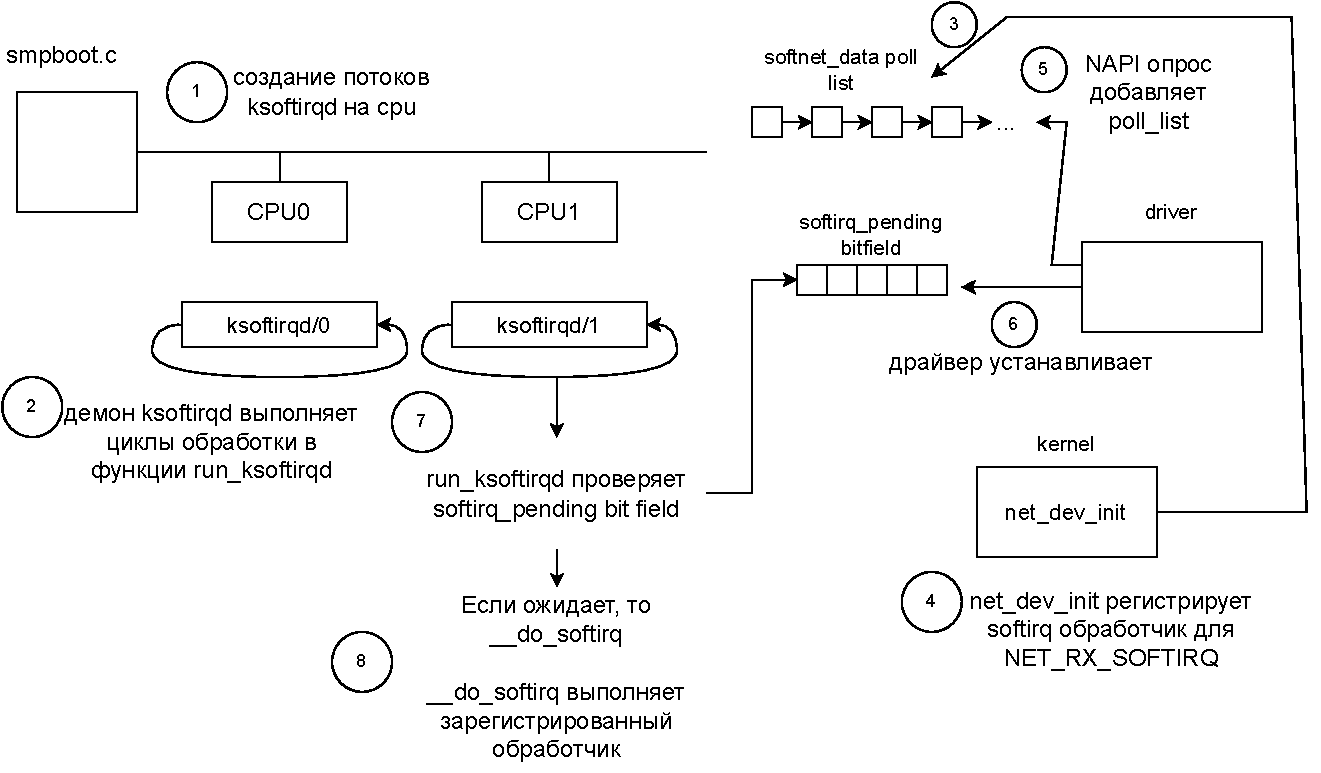
\includegraphics[width=0.8\linewidth]{./images/softirq.pdf}
  \end{tabular}
\end{table}

NAPI --- New API, появилось как ответ на возросший объем действий с сетевой подсистемой. Был разработан для улучшения выполнения высокоростных действий с сетевой подсистемой. 

High speed networking может генерировать тысячи прерываний в секунду, они должны быть обработаны.

Сначала возникшее прерывание регистрируется, затем помещается в соответствующую очередь и обрабатывается в соответствии с этой очередью

\textbf{raise\_softirq\_irqoff()}
raise\_softirq\_irqoff() помечает softirq как отложенный путем установки соответствующего бита в юитовой маске softirq (softirq pending локального процессора). Это делается в raise\_softirq().

Если при этом процессор выполняет аппаратное прерывание, то осуществляется выход из функции raise\_softirq\_irqoff() и восстанавливается флаг IF. В противном случае(если не в прерывании) вызываетс wakeup\_softirqd()

\begin{lstlisting}
  if (!n_interrupt)
            wakeup_softirqd();
\end{lstlisting}

Это объясняет, почему каждый процессор имеет собственный Ksoftirq daemon





